%{\color{Black}\hrule} -- this line is used to get line but with huge space pls find alternate
\documentclass[10pt]{report}
\usepackage[T1]{fontenc}
\usepackage[utf8]{inputenc}
\usepackage[default]{lato}
%\newcommand{\RNum}[1]{\uppercase\expandafter{\romannumeral #1\relax}}
\usepackage{titlesec} %for section underline but not implemented yet
%% If you need to pass whatever options to xcolor
%\PassOptionsToPackage{dvipsnames}{xcolor}
%\definecolor{Navy}{HTML}{000080}
%\definecolor{SlateGrey}{HTML}{2E2E2E}
%\definecolor{LightGrey}{HTML}{444444}
%\colorlet{heading}{Navy}
%\colorlet{accent}{Navy}
%\colorlet{emphasis}{SlateGrey}
%\colorlet{body}{LightGrey}

\usepackage[colorlinks]{hyperref}
\usepackage[dvipsnames]{xcolor}

%new
%\documentclass{article}

%new
\usepackage[left=2cm, right=2cm, top=2cm]{geometry}
\usepackage{graphicx}
\usepackage{url}%for adding url
\usepackage{fontawesome}%for different social media logos

\begin{document}	
%{\huge\hspace{210pt}R\'{e}sum\'{e}}
%\begin{flushleft}\huge\textbf{Bhaskar Dutt}\end{flushleft}\\\vspace{10pt}
\begin{center}\LARGE\color{BlueViolet}BHASKAR\textbf{ DUTT} \end{center}\\\vspace{10pt} 
%\\{\begin{center} \large R\'{e}sum\'{e} \end{center} }
%\\\begin{center}\noindent\rule{17.6cm}{2pt}\end{center}\\
\small\faGithub\hspace{1pt} \href{https://github.com/bhaskarsdose}{github.com/bhaskarsdose}\hspace{20pt}
\faAt\hspace{1pt} \verb"bhaskarofficial2@gmail.com"\hspace{20pt}
\faLinkedin\hspace{1pt} \href{https://www.linkedin.com/in/bhaskarsdose}{linkedin.com/in/bhaskarsdose}\hspace{20pt}
\faExternalLink\hspace{1pt} Website\\[8pt]
%\faHome\hspace{1pt} \verb"H-69c, Mansarovar Park," {\verb"Shahdara, Delhi,"} {\verb"India"}\hspace{15pt}
\hfill{\faMobile\hspace{1pt} \verb"+91-7042513094"}
%\hspace{20pt}
%\\
%{\hspace{330pt}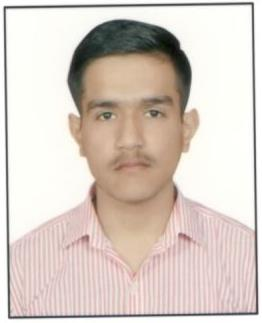
\includegraphics[scale =0.5]{bhaskar}\\[3pt]} % My image 
\section*{\color{BlueViolet}\faLightbulbO\hspace{1pt} Objective} % Details about my objective
\normalfont I am a self-motivated aspiring researcher, Tech enthusiast and a problem solver, Who always believes that perseverance beat talent, therefore, I always try to learn and implement new technologies which can help the masses. My research Interest lies in \textbf{\emph{ Mobile Computing, Embedded systems, HCI(human-computer Interaction), Wireless Networking \& ubiquitous computing.}}
% or my country. As I am always interested in the defense sector my aim is to make India reliant on its own defense equipment production and always wanted to mimic the life of Dr.APJ Abdul Kalam sir.

\section*{\color{BlueViolet}\faBook\hspace{1pt} Education} % It houses my academic performance
%\setlength\parindent{24pt} 
\textbf{B.Tech, Electrical \& Electronics Engineering, Guru Gobind Singh Indraprastha University
\hfill 2016-2020}\\
\textbf{CGPA - 8.56/10.00}\vspace{10pt}
\\
\textbf{12th C.B.S.E, Kendriya Vidyalaya, Vigyan Vihar NFC, Delhi
\hfill 2016}\\
\textbf{Overall Percentage - 87.6\%}\vspace{10pt}
\\
\textbf{10th C.B.S.E, Kendriya Vidyalaya, Vigyan Vihar NFC, Delhi
\hfill 2014}\\
\textbf{CGPA - 8.8/10}
%\begin{center}
%\begin{tabular}{|c|c|c|c|c|c|}
%	\hline
%	\hspace{2pt}\textbf{Degree} \hspace{2pt} & %\hspace{2pt}\textbf{College/School}\hspace{2pt} &\hspace{2pt} %\textbf{University}\hspace{2pt} &\hspace{2pt}\textbf{Passing Year}\hspace{2pt} & %\hspace{2pt}\textbf{Passing Percentage/CGPA}\hspace{2pt}\\
%	\hline

%	 B.Tech in EEE & ADGITM & I.P University Delhi & 2016-2020 & 8.5 \\
%	XII & K.V.N.F.C & Kendriya vidyalaya & 2004-2016 & 89\%\\
%%	\hline
%\end{tabular}
%\end{center}

\section*{\color{BlueViolet}\faLaptop\hspace{1pt} Projects}%projects has been added and updated
\noindent\textbf{\large 1. RTK Injection System Over NTRIP Server\\[1pt]}
\\\textbf{RTK or real-time kinematics} is used to enhance the precision of position data derived from satellite-based positioning systems (global navigation satellite systems, GNSS) such as GPS, GLONASS, Galileo, NavIC and BeiDou. In \textbf{drone swarming} applications this plays a very vital role for centimetre level accuracy, Built using a ublox-m8p-2 module from here+, corrections are transmitted through NTRIP caster using RTCM data packages.
\\\faExternalLink\hspace{1pt} \url{https://github.com/bhaskarsdose/RTK_Correction_Send}
\\[1pt]
 
\noindent\textbf{\large 2. LoRaWAN Based Sensor Device for IIT-D Startup\\[1pt]}
\\\textbf{Lora (Long Range)} is a low-power wide-area network (LPWAN) protocol developed by Semtech. My work includes building LoRa based sensor nodes for the device named \textbf{Ezio-statal} capable of implementing complex topologies and data transmission algorithms like \textbf{mesh, P2P, PEGASIS and LEACH}. 
\\\faExternalLink\hspace{1pt} \url{https://github.com/bhaskarsdose/Lora-Mesh}
\\[1pt]

\noindent\textbf{\large 3. Wireless Communication System For Delhi Police\\[1pt]}
\\Built a modern \textbf{walkie talkie} for Delhi police along with a \textbf{Wi-Fi Ad-hoc network} for managing law and order, Demonstrated this device at Delhi police hackathon 2019 and won 1st prize for making a working prototype among 300+ teams, Also presented demo in front of Delhi police commissioner Amulya Patnaik.
\\\faExternalLink\hspace{1pt} \url{https://github.com/bhaskarsdose/Wi-Fi-walkie-talkie-Mesh-network}
\\[1pt]


\noindent\textbf{\large 4. AR Based Autonoumous Bot - Finalist Eyrc 2019 IIT Bombay\\[1pt]}
\\In this competition, every team has a specified theme like our is a thirsty crow and there are over 28000 participants in it out of which only 150 teams were selected for the finals at IIT Bombay and our project was selected for the finals. The project includes a bot called crow which uses atmega2560 microcontroller with LFR sensor to run on black line using the command which it gets from A\* algorithm through Zigbee protocol along with that its includes use of OpenCV, OpenGL for \textbf{AR(augmented reality)}.
\\\faExternalLink\hspace{1pt} \url{https://github.com/bhaskarsdose/E-yrc-2019-crow-bot}
\\[2pt] 

\noindent\textbf{\large 5. LQR(linear–quadratic regulator) Controller Based Biped Bot\\[1pt]}
\\LQR is a feedback-based controller used in place of PID controller due to its faster response time but it requires complex mathematics in the modelling, In this project, we successfully built the model and also implemented it using 8 Bit microcontroller and controlled using Xbee based remote controller.
\\\faExternalLink\hspace{1pt} \url{https://github.com/bhaskarsdose/LQR-Bases-Self-Balancing-Bot}
\\[2pt] 


\noindent\textbf{\large 6. Real-Time Pollution Monitor For Air Quality Measurements In Industries\\[1pt] }
\\This project includes a raspberry pi device as a local server to host an MQTT server as well as a webpage to connect various nodes through mosquitto broker, on the other hand, It uses Wi-Fi capable soc to interface with sensors like bme680, a sharp dust sensor and mq135 to measure the data like temperature, pressure, humidity, AQI, NO2, SO2, CO2, PM10\&2.5 and send it to the server to log the data.
%\\\textbf{Video link:-} https://youtu.be/qMB781NHcqE
\\\faExternalLink\hspace{1pt} \url{https://github.com/bhaskarsdose/Air-Monitoring-System}           \\[2pt]
	 
\noindent\textbf{\large 7. Smart Energy Metering Device\\[1pt]}
\\This device measures and stores multiple parameters like current, voltage, frequency and temperature for purposes like energy monitoring, battery health and analytical analysis for better efficiency. 
\\\faExternalLink\hspace{1pt} \url{https://github.com/bhaskarsdose/SMART\_ENERGY\_METER}
\\[2pt]

\noindent\textbf{\large 8. Wearable For Health Monitoring \\[1pt]}
\\This project uses ThingSpeak API and a UI centric app on software stack, On sensing side a heart rate sensor on a very small Wi-Fi SOC for small footprint ideal for a wearable.
\\\faExternalLink\hspace{1pt} \url{https://github.com/bhaskarsdose/micro-health-monitoring-system}
\\[2pt]


\noindent\textbf{\large 9. Gesture Based Nano Drone\\[1pt]}
\\Currently working on this project as my major project, It uses STM based Eachine FC which receives gesture generated commands wirelessly over mavlink protocol using pi zero as a companion computer, application  \textbf{swarming, HCI and indoor navigation} 
\\\faExternalLink\hspace{1pt} \url{https://drive.google.com/file/d/1tPTBw8y6eKShXya8BZ4sjXn9a4iqKP7c/view?usp=drivesdk}
\\[1pt]

%\noindent\textbf{\large 7. Smart Socket\\[1pt]}
%\\This my internship project or mine first IoT based project from which I learnt PCB designing, relay control circuit, Nodemcu interfacing and connecting it to the internet or locally using Bluetooth hc-05 to give its command for turning on and off the appliances connected with the socket , Along with that I also integrated this with the \textbf{IFTTT} template to turn on and off the relay using the google voice assistant as it generates the instance which goes to the cloud which send the command to the applet.
%\\\textbf{Project Link:-} https://github.com/bhaskarsdose/IOT-enabled-socket
%\\[20pt]
  
\section*{\color{BlueViolet}\faSuitcase\hspace{1pt} Experience} % section for my internships
\begin{itemize}
\item{Worked as an \textbf{R\&D intern} for the embedded domain under the project \textbf{Accurate positioning using RTK in Drone swarming} at IIT Delhi under Botlab dynamics }from January 2020 to April 2020.

\hfill{\textbf{Mentor: }\textbf{Tanmay Bunkar}, Founder, Botlab Dynamics-IIT Delhi}
\item{Completed Internship at IIT Delhi incubated startup \textbf{\textit{AEROGRAM PVT. LTD.}} as an \textbf{Embedded Firmware Developer for networking devices} from August 2019 to December 2019.}

\hfill{\textbf{Mentor: }\textbf{Dr.Sarita ahlawat}, Research scientist at IIT-D \& Founder, Aerogram}
\item Worked as an \textbf{Embedded Firmware Developer Intern (IOT)} at \textbf{Algo8 PVT. LTD.}  for 6 months from January 2019 to June 2019.

\hfill{\textbf{Mentor: }\textbf{Abhinav Saksena}, CEO, Power8 (P8SENSE PVT. LTD.)}
\item Worked as an intern at \textbf{W3Dev (a startup by IIITD student)} as a junior \textbf{IOT(Internet of things)} Developer during summer of my B.Tech after 2nd semester from June 2018 to August 2018.

\hfill{\textbf{Mentor: }\textbf{Ashutosh Kumar}, Founder, W3Dev}
\item Done training on \textbf{PLC, Scada and Autocad}.
\end{itemize}

\section*{\color{BlueViolet}\faUniversity\hspace{1pt} Research Publications} %Details about research publications
\begin{itemize}
%	\item Currently working On building a standalone ad-hoc network using Wi-Fi mesh and LoRaWAN 
%	for maximizing efficiency of each node and whole system in terms of energy consumption,
%	range and data transmission rate and planning to publish paper titled \textbf{\textit{"Efficient %data transmission for an Ad-Hoc network"}}. 
	\item \textbf{[1] Bhaskar Dutt}, Gauri Goenka, Aakash Awasthi. \textbf{\textit{"Research paper:Automation in factories using Internet of Things(IoT)."}} At Journal of Emerging Technologies and Innovative Research (An International Open Access Journal) Paper ID A17, 2019 %published in the IETET journal PAPER ID \#A17.
\end{itemize}


\section*{\color{BlueViolet}\faSellsy\hspace{1pt} Technical Skills} %my technical skills AF :))))))
\begin{itemize}
\item \textbf{\emph{Technologies:}} Internet Of Things(\textbf{IoT}), Embedded systems, \textbf{Drones/autonomous vehicles}, Near sensor computing/Edge computing, AR(augmented reality), 3D modelling in Blender, PCB Designing. 
%Socket Programming, API Integration, etc.  	
\item\textbf{\emph{Programming Languages:}} C/C++, Python, \LaTeX, Embedded C   \& MATLAB/Octave.
\item\textbf{\emph{Hardware:}} TI-cc3200 LaunchXL, Arduino Uno/Mega, NodeMCU ESP-12e/ESP8266, Esp32-Wroom-32D, STM32F4xx/F2xx,\textbf{ Linux Boards-} Nvidia jetson nano, Raspberry Pi 3b/Zero, Orange pi Zero,\textbf{ Flight Controllers-} Pixhawk Px4, Matek f405 STD \& Omnibus F4 pro.
\item\textbf{\emph{Software:}} MAVproxy/Mission Planner GCS, Blender, Autodesk EAGLE, Arduino IDE, Espressif IoT Development Framework, Atmel Studio, STM32CubeIDE/TrueSTUDIO, Octave, TeXstudio, etc.
%\item Basic socket programming and API integration for IoT applications like for real world deployment.
\item\textbf{\emph{Cloud used:}}AWS IoT Core + DynamoDB, Mathworks ThingSpeak, Google's Firebase, etc.
%\item Worked on Augmented reality using openCV and openGL.
%\item Microprocessor used- Raspberry pi 3b/3b+, pi zero and Nvidia jetson nano.
%\item Technical Writing.
%\item Efficient topology and network making experience.
%\item product development ,research and designing.
%\item \textbf{LoRaWAN , Wi-Fi 802.11 Standards}  
\end{itemize}

%\section*{\color{BlueViolet}\faTasks\hspace{1pt} Soft Skills} % soft skills are here :)))))
%\begin{enumerate}
%	%\item Workaholic, Always try to complete the work given ASAP.
%	\item Ability to accept failures as I follow the saying \emph{"there are no %failures only learning".}
%	\item Time Management.
%	\item Team Management.
%	\item leadership capability.
%	\item Public speaking.
%	\item Peer to peer communication skills.
%\end{enumerate}

\section*{\color{BlueViolet}\faPencil\hspace{1pt} Extra-Curricular Activities} %extra curricular activites are here :))))
\begin{itemize}
	%\item Contributing open source projects like \textbf{Ardupilot}.
	\item Teaching Mathematics to high school students and helping juniors in various projects.
	\item A prominent reader, Loves to read a daily newspaper, Research journals , Articles \& various novels like Biographies of great personalities like Dr.APJ Abdul Kalam, Bhagat Singh, Elon Musk, Jack Ma etc.
	\item Debating.
    \item Blogging. \faExternalLink \url{bhaskarsdose.wordpress.com}
\end{itemize}

\section*{\color{BlueViolet}\faTrophy\hspace{1pt} Co-Curricular Activities}%extra curricular activities are here :)))))
\begin{enumerate}
	\item \textbf{1st Position} at \textbf{\emph{Delhi Police Hackathon 2019}}  facilitated by D.P commissioner Amulya Patnaik.
	\item Merit Certificate (All India 7th Rank) holder for \textbf{\emph{E-Yantra Robotics Competition IIT-Bombay 2018-19}} and team leader for the \textbf{only team selected for national finals} from our college (out of 28000 participants) at pan India level.
	\item Organizer of \textbf{\emph{T-HACK 2018}}, Official Hackathon of IEEE ADGITM (Formerly NIEC).
	\item Ex-Membership \& project coordinator of IEEE ADGITM (Formerly NIEC).
	\item Team lead for various Hackathon conducted across different colleges like Vihaan 2.0 DTU, IIIT Delhi Hackathon and Arduino day Hackathon of BVPCOE etc.
\end{enumerate}

%\section*{\color{BlueViolet}\faUser\hspace{1pt} Personal Details}% details for cooman use are there like names
%\textbf{Father's Name:} Mr.Narayan Dutt Sharma\\
%\textbf{Mother's Name:} Mrs.Sheela Sharma\\
%\textbf{Sex:} Male\\
%\textbf{Date Of Birth:} 16 January 1999\\
%\textbf{Nationality:} Indian\\
%\textbf{Marital Status:} Single

\section*{\color{BlueViolet}\faUsers\hspace{1pt} Mentors}%refrences are here :))))
\begin{itemize}
%\noindent 
\item\textbf{Dr.Sarita Ahlawat}, Scientist, BIRAC BIG Innovator, IIT-Delhi
\\email- sahlawat@gmail.com
\\
\item\textbf{Manoj Gulati}, Researcher, Living Analytics Research Centre (LARC)
\\email- manojg@iiitd.ac.in 
\\
\item\textbf{Anuj Barnwal}, Founder, Botlab Dynamics-IIT Delhi
\\email- anuj@botlabdynamics.com 
\end{itemize}
\\%[40pt]
%\section*{Declaration:}% resting place for declaration
%\large I hereby confirm that all the information given above is correct and I affirm that the information given above if found faulty then I owe to face any action.\\[20pt]

%\noindent\textbf{\color{BlueViolet}\faTable\hspace{1pt} \large Last Updated}\\[8pt]  
%\large May-2020% change data here
%\\[50pt] 

%\hfill\LARGE\verb|Bhaskar|
\end{document}